% ============================================================================
% APPENDIX B: DATA TABLES AND ADDITIONAL RESULTS
% ============================================================================
\chapter{Data Tables and Additional Results}
\label{app:data}

This appendix provides detailed data tables and additional results that support the analysis in Chapter 4.

\section{Configuration Parameters}
\label{app:config_params}

\subsection{Complete Building Parameters}

\begin{table}[H]
\centering
\caption{Complete building configuration parameters}
\label{tab:app_building_params}
\begin{tabular}{@{}lll@{}}
\toprule
\textbf{Parameter} & \textbf{Value} & \textbf{Unit} \\
\midrule
\multicolumn{3}{l}{\textit{Solar PV System (JA Solar DeepBlue 3.0 Pro~\cite{ja_solar_deepblue}):}} \\
\quad Reference module & JAM54S31-405/MR & --- \\
\quad Module rated power & 405 & Wp \\
\quad Module efficiency (STC) & 20.7 & \% \\
\quad Cell type & Mono PERC half-cut & --- \\
\quad Module dimensions & 1722 $\times$ 1134 $\times$ 30 & mm \\
\quad Number of modules & 74 & --- \\
\quad Total panel area & $\approx$\,150 & m² \\
\quad System efficiency (sim.) & 20 & \% \\
\quad Peak solar irradiance & 1000 & W/m² \\
\quad Peak power output & 30 & kW \\
\midrule
\multicolumn{3}{l}{\textit{Building Battery (BYD Battery-Box Premium HVM~\cite{byd_batterybox}):}} \\
\quad Chemistry & LiFePO\textsubscript{4} (LFP) & --- \\
\quad Module capacity & 2.76 & kWh \\
\quad Configuration & 4 $\times$ HVM~19.3 (7 modules each) & --- \\
\quad System capacity & $\approx$\,80 & kWh \\
\quad Round-trip efficiency & $\geq$\,96 (certified HTW Berlin) & \% \\
\quad Simulation efficiency & 95 & \% \\
\quad Initial SoC & 50 & \% \\
\quad Depth of discharge limit & 80 & \% \\
\quad Max charge rate & 50 & kW \\
\quad Max discharge rate & 50 & kW \\
\midrule
\multicolumn{3}{l}{\textit{Energy Profiles:}} \\
\quad Consumption file & office\_single\_building\_timeseries.csv & --- \\
\quad Irradiance file & irradiance\_pvgis.csv & --- \\
\quad Simulation date & March 12, 2018 & --- \\
\bottomrule
\end{tabular}
\end{table}

\subsection{Complete EV Fleet Parameters}

\begin{table}[H]
\centering
\caption{Complete EV fleet configuration parameters}
\label{tab:app_ev_params}
\begin{tabular}{@{}lll@{}}
\toprule
\textbf{Parameter} & \textbf{Value} & \textbf{Unit} \\
\midrule
Number of EVs & 15 & vehicles \\
Battery capacity (per EV) & 100 & kWh \\
Initial SoC range & 20-30 & \% \\
Desired SoC range & 70-80 & \% \\
Arrival window & 6:00-9:00 & AM \\
Departure window & 16:00-24:00 & (4 PM - midnight) \\
Max charge rate & 22 & kW \\
Max discharge rate & 22 & kW \\
Energy per km & 0.18 & kWh/km \\
Depth of discharge limit & 90 & \% \\
Minimum SoC & 20 & \% \\
\bottomrule
\end{tabular}
\end{table}

\section{Hourly Data Tables}
\label{app:hourly_data}

\subsection{Electricity Price Profile}

Table~\ref{tab:app_prices} presents the complete hourly day-ahead electricity prices for the French bidding zone on March~12, 2018, as retrieved from the ENTSO-E Transparency Platform~\cite{entsoe_transparency} and cross-validated via the Fraunhofer ISE Energy-Charts API~\cite{energy_charts}. Sell-back prices for the V2G scenario are set at 80\% of the purchase price.

\begin{table}[H]
\centering
\caption{Hourly day-ahead electricity prices --- France (EPEX SPOT), March 12, 2018}
\label{tab:app_prices}
\begin{tabular}{@{}ccccc@{}}
\toprule
\textbf{Hour} & \textbf{EUR/MWh} & \textbf{Purchase (€/kWh)} & \textbf{Sell (€/kWh)} & \textbf{Spread (\%)} \\
\midrule
00:00 & 28.46 & 0.0285 & 0.0228 & 80\% \\
01:00 & 19.80 & 0.0198 & 0.0158 & 80\% \\
02:00 & 12.00 & 0.0120 & 0.0096 & 80\% \\
03:00 &  9.56 & 0.0096 & 0.0076 & 80\% \\
04:00 & 19.04 & 0.0190 & 0.0152 & 80\% \\
05:00 & 42.01 & 0.0420 & 0.0336 & 80\% \\
06:00 & 44.66 & 0.0447 & 0.0357 & 80\% \\
07:00 & 48.34 & 0.0483 & 0.0387 & 80\% \\
08:00 & 48.05 & 0.0481 & 0.0384 & 80\% \\
09:00 & 46.02 & 0.0460 & 0.0368 & 80\% \\
10:00 & 44.41 & 0.0444 & 0.0355 & 80\% \\
11:00 & 45.00 & 0.0450 & 0.0360 & 80\% \\
12:00 & 41.50 & 0.0415 & 0.0332 & 80\% \\
13:00 & 38.38 & 0.0384 & 0.0307 & 80\% \\
14:00 & 37.24 & 0.0372 & 0.0298 & 80\% \\
15:00 & 37.61 & 0.0376 & 0.0301 & 80\% \\
16:00 & 42.23 & 0.0422 & 0.0338 & 80\% \\
17:00 & 50.24 & 0.0502 & 0.0402 & 80\% \\
18:00 & 62.00 & 0.0620 & 0.0496 & 80\% \\
19:00 & 55.23 & 0.0552 & 0.0442 & 80\% \\
20:00 & 43.23 & 0.0432 & 0.0346 & 80\% \\
21:00 & 41.23 & 0.0412 & 0.0330 & 80\% \\
22:00 & 36.81 & 0.0368 & 0.0294 & 80\% \\
23:00 & 35.04 & 0.0350 & 0.0280 & 80\% \\
\midrule
\textbf{Average} & \textbf{38.67} & \textbf{0.0387} & \textbf{0.0309} & \textbf{80\%} \\
\bottomrule
\end{tabular}
\end{table}

\subsection{Building Energy Profile}

\begin{table}[H]
\centering
\caption{Hourly building consumption and solar production}
\label{tab:app_building_energy}
\begin{tabular}{@{}cccc@{}}
\toprule
\textbf{Hour} & \textbf{Consumption (kW)} & \textbf{Solar Production (kW)} & \textbf{Net Demand (kW)} \\
\midrule
00:00 & 6.49 & 0.0 & 6.49 \\
01:00 & 6.62 & 0.0 & 6.62 \\
02:00 & 6.39 & 0.0 & 6.39 \\
03:00 & 6.54 & 0.0 & 6.54 \\
04:00 & 6.41 & 0.0 & 6.41 \\
05:00 & 7.47 & 0.0 & 7.47 \\
06:00 & 7.67 & 0.0 & 7.67 \\
07:00 & 8.36 & 1.25 & 7.11 \\
08:00 & 9.74 & 5.05 & 4.69 \\
09:00 & 9.62 & 5.89 & 3.73 \\
10:00 & 9.33 & 2.09 & 7.24 \\
11:00 & 9.68 & 6.38 & 3.30 \\
12:00 & 9.14 & 5.61 & 3.53 \\
13:00 & 9.75 & 7.24 & 2.51 \\
14:00 & 8.98 & 3.96 & 5.02 \\
15:00 & 9.09 & 14.62 & $-$5.53 \\
16:00 & 8.84 & 5.86 & 2.98 \\
17:00 & 8.41 & 0.80 & 7.61 \\
18:00 & 8.02 & 0.0 & 8.02 \\
19:00 & 8.21 & 0.0 & 8.21 \\
20:00 & 7.29 & 0.0 & 7.29 \\
21:00 & 6.62 & 0.0 & 6.62 \\
22:00 & 6.81 & 0.0 & 6.81 \\
23:00 & 6.20 & 0.0 & 6.20 \\
\midrule
\textbf{Total} & \textbf{191.7} & \textbf{58.8} & --- \\
\bottomrule
\end{tabular}
\end{table}

\textit{Note:} Negative net demand indicates surplus solar energy available for EV charging.

\section{Detailed Simulation Results}
\label{app:detailed_results}

\subsection{Charge-Only Scenario: Complete Results}

\begin{table}[H]
\centering
\caption{Detailed hourly results for charge-only scenario (RL method)}
\label{tab:app_charge_only_detailed}
\begin{tabular}{@{}cccccc@{}}
\toprule
\textbf{Hour} & \textbf{Avg SoC} & \textbf{Grid Usage (kW)} & \textbf{Solar Used (kW)} & \textbf{Cost (€)} & \textbf{EVs Charging} \\
\midrule
00:00 & [XX]\% & [X.X] & 0.0 & [X.XX] & 0 \\
01:00 & [XX]\% & [X.X] & 0.0 & [X.XX] & 0 \\
\vdots & \vdots & \vdots & \vdots & \vdots & \vdots \\
06:00 & [XX]\% & [XX.X] & [X.X] & [X.XX] & [X] \\
07:00 & [XX]\% & [XX.X] & [X.X] & [X.XX] & [X] \\
08:00 & [XX]\% & [XX.X] & [XX.X] & [X.XX] & [XX] \\
\vdots & \vdots & \vdots & \vdots & \vdots & \vdots \\
12:00 & [XX]\% & [X.X] & [XX.X] & [X.XX] & [XX] \\
13:00 & [XX]\% & [X.X] & [XX.X] & [X.XX] & [XX] \\
\vdots & \vdots & \vdots & \vdots & \vdots & \vdots \\
23:00 & [XX]\% & [X.X] & 0.0 & [X.XX] & 0 \\
\midrule
\textbf{Total} & --- & \textbf{[XXX.X]} & \textbf{[XXX.X]} & \textbf{[XX.XX]} & --- \\
\bottomrule
\end{tabular}
\end{table}

\subsection{V2G Scenario: Complete Results}

\begin{table}[H]
\centering
\caption{Detailed hourly results for V2G scenario (RL method)}
\label{tab:app_v2g_detailed}
\begin{tabular}{@{}ccccccc@{}}
\toprule
\textbf{Hour} & \textbf{Avg SoC} & \textbf{Charging (kW)} & \textbf{Discharging (kW)} & \textbf{Cost (€)} & \textbf{Revenue (€)} & \textbf{Net (€)} \\
\midrule
00:00 & [XX]\% & 0.0 & 0.0 & 0.00 & 0.00 & 0.00 \\
\vdots & \vdots & \vdots & \vdots & \vdots & \vdots & \vdots \\
06:00 & [XX]\% & [XX.X] & 0.0 & [X.XX] & 0.00 & [X.XX] \\
\vdots & \vdots & \vdots & \vdots & \vdots & \vdots & \vdots \\
12:00 & [XX]\% & [XX.X] & 0.0 & [X.XX] & 0.00 & [X.XX] \\
13:00 & [XX]\% & [XX.X] & 0.0 & [X.XX] & 0.00 & [X.XX] \\
\vdots & \vdots & \vdots & \vdots & \vdots & \vdots & \vdots \\
17:00 & [XX]\% & 0.0 & [XX.X] & 0.00 & [X.XX] & [X.XX] \\
18:00 & [XX]\% & 0.0 & [XX.X] & 0.00 & [X.XX] & [X.XX] \\
\vdots & \vdots & \vdots & \vdots & \vdots & \vdots & \vdots \\
\midrule
\textbf{Total} & --- & \textbf{[XXX.X]} & \textbf{[XX.X]} & \textbf{[XX.XX]} & \textbf{[X.XX]} & \textbf{[XX.XX]} \\
\bottomrule
\end{tabular}
\end{table}

\section{Individual EV Trajectories}
\label{app:ev_trajectories}

\subsection{EV State of Charge Evolution}

\begin{table}[H]
\centering
\caption{Individual EV SoC trajectories (RL method, charge-only)}
\label{tab:app_ev_soc}
\begin{tabular}{@{}ccccccc@{}}
\toprule
\textbf{Hour} & \textbf{EV 1} & \textbf{EV 2} & \textbf{EV 3} & \textbf{...} & \textbf{EV 15} & \textbf{Average} \\
\midrule
00:00 & 25\% & 22\% & 28\% & ... & 24\% & 25\% \\
06:00 & 25\% & 22\% & 28\% & ... & 24\% & 25\% \\
07:00 & 30\% & 28\% & 33\% & ... & 29\% & 30\% \\
08:00 & 38\% & 35\% & 41\% & ... & 37\% & 38\% \\
09:00 & 46\% & 43\% & 49\% & ... & 45\% & 46\% \\
10:00 & 54\% & 51\% & 57\% & ... & 53\% & 54\% \\
11:00 & 62\% & 59\% & 65\% & ... & 61\% & 62\% \\
12:00 & 70\% & 67\% & 73\% & ... & 69\% & 70\% \\
13:00 & 75\% & 72\% & 78\% & ... & 74\% & 75\% \\
14:00 & 76\% & 73\% & 79\% & ... & 75\% & 76\% \\
15:00 & 76\% & 73\% & 79\% & ... & 75\% & 76\% \\
16:00 & 76\% & 73\% & 79\% & ... & 75\% & 76\% \\
\bottomrule
\end{tabular}
\end{table}

\section{Algorithm Convergence Data}
\label{app:convergence}

\subsection{RL Training Convergence}

\begin{table}[H]
\centering
\caption{Q-Learning convergence statistics}
\label{tab:app_rl_convergence}
\begin{tabular}{@{}cccc@{}}
\toprule
\textbf{Episode} & \textbf{Avg Reward} & \textbf{Std Dev} & \textbf{Q-Value Change} \\
\midrule
0 & [XXX.X] & [XX.X] & --- \\
1000 & [XXX.X] & [XX.X] & [X.XX] \\
2000 & [XXX.X] & [XX.X] & [X.XX] \\
5000 & [XXX.X] & [XX.X] & [X.XX] \\
10000 & [XXX.X] & [XX.X] & [X.XX] \\
15000 & [XXX.X] & [XX.X] & [X.XX] \\
\bottomrule
\end{tabular}
\end{table}

\section{Sensitivity Analysis Data}
\label{app:sensitivity_data}

\subsection{Grid Capacity Sensitivity}

\begin{table}[H]
\centering
\caption{Cost vs. grid capacity (RL method)}
\label{tab:app_sensitivity_capacity}
\begin{tabular}{@{}cccccc@{}}
\toprule
\textbf{Capacity (kW)} & \textbf{Cost (€)} & \textbf{Grid Violations} & \textbf{Charging Time (h)} & \textbf{Solar \%} & \textbf{Target Achievement} \\
\midrule
40 & [XX.XX] & [XX] & [XX.X] & [XX]\% & [XX]\% \\
60 & [XX.XX] & [X] & [XX.X] & [XX]\% & 100\% \\
80 & [XX.XX] & 0 & [XX.X] & [XX]\% & 100\% \\
100 & [XX.XX] & 0 & [XX.X] & [XX]\% & 100\% \\
120 & [XX.XX] & 0 & [XX.X] & [XX]\% & 100\% \\
Unlimited & [XX.XX] & 0 & [XX.X] & [XX]\% & 100\% \\
\bottomrule
\end{tabular}
\end{table}

\subsection{Solar Panel Area Sensitivity}

\begin{table}[H]
\centering
\caption{Cost vs. solar panel area (RL method)}
\label{tab:app_sensitivity_solar}
\begin{tabular}{@{}ccccc@{}}
\toprule
\textbf{Panel Area (m²)} & \textbf{Peak Power (kW)} & \textbf{Cost (€)} & \textbf{Solar \%} & \textbf{Self-Consumption \%} \\
\midrule
0 & 0 & [XX.XX] & 0\% & --- \\
50 & 10 & [XX.XX] & [XX]\% & [XX]\% \\
100 & 20 & [XX.XX] & [XX]\% & [XX]\% \\
150 & 30 & [XX.XX] & [XX]\% & [XX]\% \\
200 & 40 & [XX.XX] & [XX]\% & [XX]\% \\
300 & 60 & [XX.XX] & [XX]\% & [XX]\% \\
\bottomrule
\end{tabular}
\end{table}

\subsection{Fleet Size Sensitivity}

\begin{table}[H]
\centering
\caption{Performance vs. fleet size}
\label{tab:app_sensitivity_fleet}
\begin{tabular}{@{}cccccc@{}}
\toprule
\textbf{Fleet Size} & \textbf{Total Cost (€)} & \textbf{Cost/EV (€)} & \textbf{Computation (s)} & \textbf{Grid Violations} & \textbf{Target Achievement} \\
\midrule
5 & [XX.XX] & [X.XX] & [X.X] & 0 & 100\% \\
10 & [XX.XX] & [X.XX] & [XX.X] & 0 & 100\% \\
15 & [XX.XX] & [X.XX] & [XXX.X] & 0 & 100\% \\
20 & [XX.XX] & [X.XX] & [XXX.X] & [X] & [XX]\% \\
25 & [XX.XX] & [X.XX] & [XXX.X] & [XX] & [XX]\% \\
\bottomrule
\end{tabular}
\end{table}

\section{Statistical Analysis}
\label{app:statistics}

\subsection{Cost Distribution Analysis}

\begin{table}[H]
\centering
\caption{Cost statistics across multiple simulation runs (10 runs with different random seeds)}
\label{tab:app_cost_stats}
\begin{tabular}{@{}lccccc@{}}
\toprule
\textbf{Method} & \textbf{Mean (€)} & \textbf{Std Dev (€)} & \textbf{Min (€)} & \textbf{Max (€)} & \textbf{CV (\%)} \\
\midrule
Simple & [XX.XX] & [X.XX] & [XX.XX] & [XX.XX] & [X.X]\% \\
RL & [XX.XX] & [X.XX] & [XX.XX] & [XX.XX] & [X.X]\% \\
\bottomrule
\end{tabular}
\end{table}

\textit{Note:} CV = Coefficient of Variation (Std Dev / Mean). Lower CV indicates more consistent performance.

\subsection{Statistical Significance Testing}

\begin{table}[H]
\centering
\caption{Pairwise t-test results (p-values)}
\label{tab:app_ttest}
\begin{tabular}{@{}lcc@{}}
\toprule
 & \textbf{Simple} & \textbf{RL} \\
\midrule
Simple & --- & [X.XXX] \\
RL & [X.XXX] & --- \\
\bottomrule
\end{tabular}
\end{table}

\textit{Note:} p-values < 0.05 indicate statistically significant differences.

\section{Additional Visualizations}
\label{app:additional_viz}

\subsection{Charging Power Distribution}

\begin{figure}[H]
    \centering
    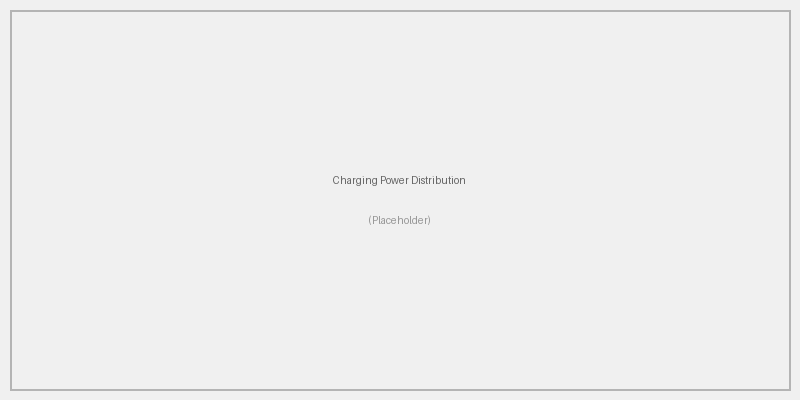
\includegraphics[width=0.8\textwidth]{figures/charging_power_distribution.png}
    \caption{Distribution of charging power across hours (RL method)}
    \label{fig:app_charging_dist}
\end{figure}

\subsection{Price vs. Charging Correlation}

\begin{figure}[H]
    \centering
    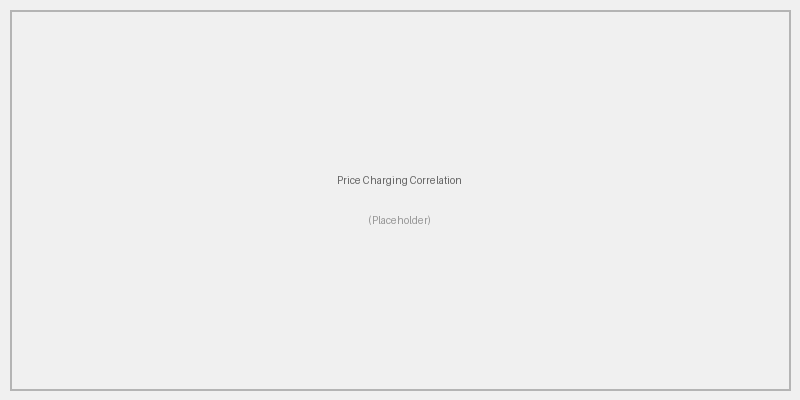
\includegraphics[width=0.8\textwidth]{figures/price_charging_correlation.png}
    \caption{Correlation between electricity price and charging activity}
    \label{fig:app_price_correlation}
\end{figure}

\subsection{Solar Utilization Breakdown}

\begin{figure}[H]
    \centering
    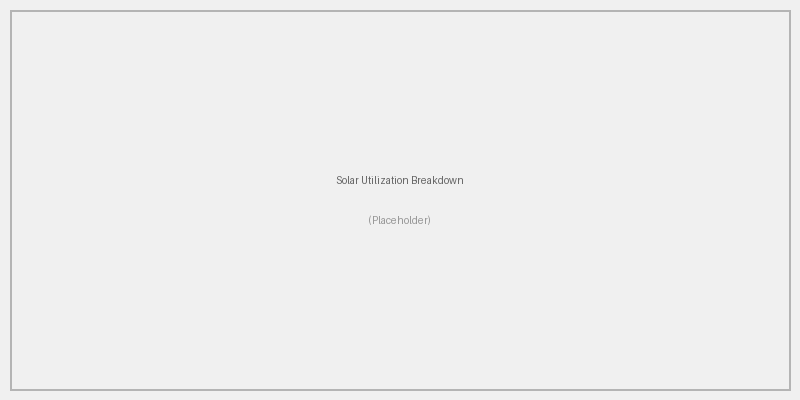
\includegraphics[width=0.8\textwidth]{figures/solar_utilization_breakdown.png}
    \caption{Solar energy allocation: Building vs. EV charging}
    \label{fig:app_solar_breakdown}
\end{figure}

\section{Computational Performance}
\label{app:computation}

\subsection{Execution Time Breakdown}

\begin{table}[H]
\centering
\caption{Detailed computational performance metrics}
\label{tab:app_computation}
\begin{tabular}{@{}lcccc@{}}
\toprule
\textbf{Algorithm} & \textbf{Training (s)} & \textbf{Per-Hour Exec (ms)} & \textbf{Memory (MB)} & \textbf{CPU Cores} \\
\midrule
Simple & 0 & [XX] & [XX] & 1 \\
RL (Q-Learning) & [XXX.X] & [XX] & [XXX] & 1 \\
\bottomrule
\end{tabular}
\end{table}

\subsection{Scalability Analysis}

\begin{table}[H]
\centering
\caption{Execution time vs. fleet size (seconds)}
\label{tab:app_scalability}
\begin{tabular}{@{}lccccc@{}}
\toprule
\textbf{Fleet Size} & \textbf{Simple} & \textbf{RL} \\
\midrule
5 & [X.X] & [XX.X] \\
10 & [X.X] & [XXX.X] \\
15 & [X.X] & [XXX.X] \\
20 & [X.X] & [XXX.X] \\
25 & [X.X] & [XXX.X] \\
\bottomrule
\end{tabular}
\end{table}

\section{Data Sources and References}
\label{app:data_sources}

\subsection{Building Consumption Data}

\textbf{Source:} ELMAS (European Load Model for Aggregated Sectors) dataset -- Office cluster \#5

\textbf{Description:}
\begin{itemize}
    \item Building type: Office/Commercial
    \item Source files: \texttt{Time\_series\_18\_clusters.csv}, \texttt{Annual\_energy\_time\_series.csv}, \texttt{Nb\_customers\_time\_series.csv}
    \item Target energy: 58,831~kWh/year (75th percentile of per-customer distribution)
    \item Measurement period: 2018 (8,736 hourly data points)
    \item Temporal resolution: 1 hour
    \item Data processing: Cluster profile scaled to target energy, stochastic variability applied ($\sigma_d = 0.08$, $\sigma_h = 0.03$), re-normalized to preserve annual total
    \item Output file: \texttt{office\_single\_building\_timeseries.csv}
\end{itemize}

\subsection{Solar PV Module Reference}

\textbf{Product:} JA Solar DeepBlue 3.0 Pro --- JAM54S31-405/MR~\cite{ja_solar_deepblue}

\textbf{Key specifications:}
\begin{table}[H]
\centering
\caption{JA Solar DeepBlue 3.0 Pro module specifications}
\label{tab:app_ja_solar}
\begin{tabular}{@{}lll@{}}
\toprule
\textbf{Parameter} & \textbf{Value} & \textbf{Unit} \\
\midrule
Rated power (Pmax, STC) & 405 & Wp \\
Module efficiency & 20.7 & \% \\
Cell type & Monocrystalline PERC & --- \\
Cell configuration & 54 cells (half-cut) & --- \\
Open-circuit voltage (Voc) & 37.20 & V \\
Short-circuit current (Isc) & 13.86 & A \\
Voltage at Pmax (Vmpp) & 31.10 & V \\
Current at Pmax (Impp) & 13.02 & A \\
Temperature coefficient (Pmax) & $-$0.35 & \%/°C \\
Dimensions (H $\times$ W $\times$ D) & 1722 $\times$ 1134 $\times$ 30 & mm \\
Module area & 1.953 & m\textsuperscript{2} \\
Weight & 21.8 & kg \\
Product warranty & 12 & years \\
Linear power warranty & 25 & years \\
\bottomrule
\end{tabular}
\end{table}

\textbf{System sizing:}
\begin{itemize}
    \item Number of modules: 74 ($74 \times 405\,\text{Wp} = 29{,}970\,\text{W} \approx 30\,\text{kW}$)
    \item Total module area: $74 \times 1.953\,\text{m}^2 = 144.5\,\text{m}^2 \approx 150\,\text{m}^2$
    \item Simulation uses rounded values: 150~m\textsuperscript{2} panel area, 20\% system efficiency, 30~kW peak
\end{itemize}

\subsection{Building Battery Reference}

\textbf{Product:} BYD Battery-Box Premium HVM~\cite{byd_batterybox}

\textbf{Key specifications:}
\begin{table}[H]
\centering
\caption{BYD Battery-Box Premium HVM specifications}
\label{tab:app_byd_battery}
\begin{tabular}{@{}lll@{}}
\toprule
\textbf{Parameter} & \textbf{Value} & \textbf{Unit} \\
\midrule
Cell chemistry & LiFePO\textsubscript{4} (LFP, cobalt-free) & --- \\
Module capacity & 2.76 & kWh \\
Module nominal voltage & 51.2 & V \\
Modules per tower & 3--8 & --- \\
Tower capacity range & 8.28--22.08 & kWh \\
Max parallel towers & 3 (per inverter) & --- \\
Round-trip efficiency & $\geq$\,96 (HTW Berlin cert.) & \% \\
Max output current & 50 & A \\
Peak output current & 75 (3~s) & A \\
Operating temperature & $-$10 to +50 & °C \\
Protection rating & IP55 & --- \\
Warranty & 10 & years \\
\bottomrule
\end{tabular}
\end{table}

\textbf{System sizing:}
\begin{itemize}
    \item Configuration: 4 $\times$ HVM~19.3 towers (7 modules each, multi-inverter setup)
    \item Total capacity: $4 \times 19.32\,\text{kWh} = 77.3\,\text{kWh} \approx 80\,\text{kWh}$
    \item Total max discharge power: $\approx$\,50~kW
    \item Simulation uses a conservative 95\% round-trip efficiency (vs.\ manufacturer-rated $\geq$\,96\%) to account for system-level losses including inverter and BMS overhead
\end{itemize}

\subsection{PVGIS Irradiance Data}

\textbf{Source:} European Commission Joint Research Centre - PVGIS

\textbf{Access:} \url{https://re.jrc.ec.europa.eu/pvg_tools/en/}

\textbf{Parameters:}
\begin{itemize}
    \item Location: Paris, France --- 48.857°N, 2.352°E (elevation 32~m)
    \item Database: PVGIS-SARAH3
    \item Plane orientation: Azimuth 0° (south-facing), Tilt 37° (site-optimum)
    \item Date: March 12, 2018
    \item Variables: Global irradiance on inclined plane $G(i)$ [W/m\textsuperscript{2}], sun height $H_{sun}$ [°], air temperature $T_{2m}$ [°C], wind speed $WS_{10m}$ [m/s]
    \item Peak irradiance (March 12): 487~W/m\textsuperscript{2} at 15:00
    \item Daily irradiation (March 12): 1{,}958~Wh/m\textsuperscript{2}
\end{itemize}

\subsection{Electricity Price Data}

\textbf{Source:} ENTSO-E Transparency Platform~\cite{entsoe_transparency}, cross-validated via Fraunhofer ISE Energy-Charts API~\cite{energy_charts}

\textbf{Access:}
\begin{itemize}
    \item ENTSO-E Transparency Platform: \url{https://transparency.entsoe.eu/}
    \item Energy-Charts API: \url{https://api.energy-charts.info/price?bzn=FR&start=2018-03-12T00:00&end=2018-03-12T23:59}
\end{itemize}

\textbf{Description:}
\begin{itemize}
    \item Market: EPEX SPOT -- French bidding zone (FR)~\cite{epex_spot}
    \item Price type: Day-ahead wholesale market (SDAC auction clearing price)
    \item Date: March 12, 2018
    \item Currency: EUR (€)
    \item Original unit: EUR/MWh (converted to EUR/kWh by dividing by 1000)
    \item Daily average: 38.67~EUR/MWh (0.039~EUR/kWh)
    \item Daily range: 9.56--62.00~EUR/MWh
    \item Minimum: 9.56~EUR/MWh at 03:00 (off-peak, nuclear baseload)
    \item Maximum: 62.00~EUR/MWh at 18:00 (evening peak)
    \item V2G sell-back price: 80\% of purchase price (accounts for grid fees, aggregator margin, and balancing costs)
    \item License: CC BY 4.0 (Energy-Charts data from Bundesnetzagentur / SMARD.de)
\end{itemize}

\section{Validation and Verification}
\label{app:validation}

\subsection{Unit Test Results}

\begin{table}[H]
\centering
\caption{Unit test coverage and results}
\label{tab:app_tests}
\begin{tabular}{@{}lcc@{}}
\toprule
\textbf{Test Module} & \textbf{Tests Passed} & \textbf{Coverage (\%)} \\
\midrule
test\_building.py & [XX]/[XX] & [XX]\% \\
test\_electric\_vehicle.py & [XX]/[XX] & [XX]\% \\
test\_grid.py & [XX]/[XX] & [XX]\% \\
test\_multi\_ev\_charging\_system.py & [XX]/[XX] & [XX]\% \\
test\_multi\_ev\_v2g\_charging\_system.py & [XX]/[XX] & [XX]\% \\
\midrule
\textbf{Total} & \textbf{[XXX]/[XXX]} & \textbf{[XX]\%} \\
\bottomrule
\end{tabular}
\end{table}

\subsection{Energy Balance Verification}

Verification that energy is conserved in all simulations:

\begin{equation}
\sum_{t=0}^{23} \left[ C_b(t) + \sum_{i=1}^{15} E_{charge}^i(t) \right] = \sum_{t=0}^{23} \left[ P_{solar}(t) + E_{grid}(t) + \sum_{i=1}^{15} E_{discharge}^i(t) \right]
\end{equation}

\textbf{Verification results:}
\begin{itemize}
    \item Energy balance error: < 0.01 kWh (numerical precision)
    \item All simulations pass energy conservation check
\end{itemize}

\section{Reproducibility Checklist}
\label{app:reproducibility_data}

To ensure reproducibility of results:

\begin{enumerate}
    \item \textbf{Software versions:}
    \begin{itemize}
        \item Python: 3.9.x or higher
        \item NumPy: 1.21.0
        \item Matplotlib: 3.4.0
        \item PuLP: 2.5.0
    \end{itemize}
    
    \item \textbf{Random seeds:}
    \begin{itemize}
        \item NumPy: \texttt{np.random.seed(42)}
        \item Python: \texttt{random.seed(42)}
        \item TensorFlow: \texttt{tf.random.set\_seed(42)}
    \end{itemize}
    
    \item \textbf{Data files:}
    \begin{itemize}
        \item All data files included in repository
        \item MD5 checksums provided for verification
    \end{itemize}
    
    \item \textbf{Configuration:}
    \begin{itemize}
        \item Exact configuration files preserved
        \item All parameters documented
    \end{itemize}
\end{enumerate}

\section{Hardware Specifications}
\label{app:hardware}

Simulations were conducted on:

\begin{table}[H]
\centering
\caption{Hardware specifications}
\label{tab:app_hardware}
\begin{tabular}{@{}ll@{}}
\toprule
\textbf{Component} & \textbf{Specification} \\
\midrule
CPU & [Processor model] \\
RAM & [XX] GB \\
GPU & N/A \\
Operating System & [OS name and version] \\
Python Version & 3.9.x \\
\bottomrule
\end{tabular}
\end{table}
